% !TEX root = main.tex
\section{Technical Overview}
\begin{frame}{Notations}
	$\R = \ZZ[X] / \generation{X^N + 1}$ where $N = 2^k$ for some $k \in \NN$.
	
	Let $Q = \prod_{i = 0}^L q_i$ be a product of primes.
	
	$\R_Q = \ZZ_Q[X]/ \generation{X^N + 1}$.
	
	Ciphertext $\bc \in \R_Q^u$ is $\bc(Y) = c_0 + c_1 \cdot Y + \dots + c_{u - 1} \cdot Y^{u-1}$.
\end{frame}

\begin{frame}{Encryption, Decryption and Evaluations}
	The construction follows BGV \cite{ITCS:BraGenVai12}.
	
	Ciphertexts $c_0(Y) = a_0\cdot Y + b_0$ and $c_1(Y) = a_1 \cdot Y + b_1$.
	
	\textbf{Addition:} $c_\add(Y) = c_0(Y) + c_1(Y) = (a_0 + a_1)\cdot Y + (b_0 + b_1)$.
	
	\textbf{Multiplication:} $c_\mult(Y) = c_0(Y)\cdot c_1(Y) = a_0\cdot a_1 \cdot Y^2 + (a_0\cdot b_1 + a_1 \cdot b_0) \cdot Y + b_0\cdot b_1$.
	
	$\Rightarrow$ \textbf{Issue:} Noise growth.
	
\end{frame}

\begin{frame}{Chinese Remaindering Theorem}
	Large $Q = \prod_{i = 0}^L q_i$.
	
	Use Chinese remainder theorem
	\begin{equation*}
		\R_Q = \frac{\ZZ_Q[X]}{\generation{X^N + 1}} \cong \prod_{i = 0}^L \frac{\ZZ_{q_i}[X]}{\generation{X^N + 1}}
	\end{equation*}
	
	Fast multiplications of polynomials can be proceeded by using number-theoretic transform (NTT).
\end{frame}

\begin{frame}{Chinese Remaindering Theorem (Continued)}
	\begin{figure}
		\centering
		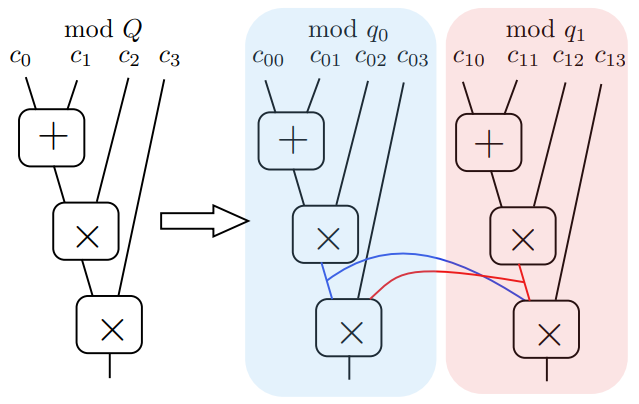
\includegraphics[width=1\linewidth]{CRT}
		\caption{Handling with CRT (Figure 1 in \cite{CIC:ABPS24}).}
		\label{fig:crt}
	\end{figure}
	
\end{frame}

\begin{frame}{Relinearization}
	\textbf{Purpose:} $c(Y) = c_0 + c_1 \cdot Y + c_2 \cdot Y^2 \Rightarrow c'(Y) = c'_0 + c'_1 \cdot Y$.
	
	\textbf{Method:}
	\begin{itemize}
		\item Encrypt $\sk^2$ as $\rlk(Y) = \rlk_0 + \rlk_1 \cdot Y$. 
		\item Compute $c'_j = c_j + c_2 \cdot \rlk_j$ for $j \in \{0,1\}$.
	\end{itemize} 
	
	$\Rightarrow$ This may incurs a large noise term.
	
	\textbf{Alternative method:} Decompose $c_2$ into RNS base by using fast base extension $\FastBaseExt$ and view $\rlk_0, \rlk_1$ as vectors. Then, compute $c'_j = c_j + \innerproduct{\D_{Q^{(i)}}(c_2)}{\rlk_j}$ for $j \in \{0,1\}$.
\end{frame}

\begin{frame}{Modulus Switching}
	Let $Q^{(k)} = \prod_{j = 0}^k q_j$.
	
	For ciphertext $c(Y) \in \R_{Q^{(i)}}[Y]$, switch to the ciphertext $c'(Y) \in \R_{Q^{(i-1)}}[Y]$ where $Q^{(i-1)} = Q^{(i)} / q_i$ s.t. $c(Y)$ and $c'(Y)$ are equivalent modulo $t$.
	
	Let $c(Y) = c_0 + c_1\cdot Y$.
	
	Then, $c'(Y) = c'_0 + c'_1 \cdot Y$ where $c'_l = (c_l + \delta_l)/q_i$ where $\delta_l = t (-c_l/t \mod q_i)$ for $l \in \{0,1\}$.
\end{frame}